\documentclass[a4paper,11pt]{article}
\usepackage[margin=2cm]{geometry}
\usepackage{anysize}
\usepackage[pdftex]{graphicx}
\usepackage{url}
\usepackage{listings}
\usepackage{textcomp}
\usepackage{wrapfig}
\usepackage{color}
\usepackage{fancyhdr}
\usepackage[nodayofweek]{datetime}
\longdate

\setlength{\parskip}{10pt} 
\setlength\parindent{0pt}
\pagestyle{fancyplain}
\fancyhf{}
\lhead{\fancyplain{}{M.Sc.\ Group Project Report}}
\rhead{\fancyplain{}{\today}}
\cfoot{\fancyplain{}{\thepage}}


\title{Twitter for traffic\\\Large{--- Report One ---}}
\author{Porfyrios Vasileiou, Marianna Polatoglou, Afxentios Hadjiminas,\\
        Panagiotis Tsirigotis, Hanguang Zhou, John Flanagan.\\
       \{pv311, mp1911, ah2411, pt1111, hz511, jf311.\}@doc.ic.ac.uk\\ \\
       \small{Supervisor: Dr.\ Emil Lupu, Dr.\ Alessandra Russo, Luke Dickens}\\
       \small{Course: CO533, Imperial College London}
}



%Report details http://www.doc.ic.ac.uk/~cristic/teaching/MScGroupProj/

\begin{document}
\maketitle

\section{Introduction}
	Twitter for traffic aims to provide the mobile user with an application for assessing traffic disruptions as they evolve. To provide this insight, the application will present the user with curated traffic disruptions augmented with social knowledge of the event harvested from a social network. In addition to this curated list of traffic disruptions, Twitter for traffic will also extract clusters of disruption reports from social networks to identify new disruptions.

To successfully achieve the project goals, the development will encompass an understanding from many areas of computer science. Aspects of this project include data mining, social network analysis, mobile application development, document classification and geographical information systems. Analysing the social and curated datafeeds to identify new disruption events will be a particularly interesting undertaking. From the onset there are many unknowns relating to the data analysis, relating to the quantity of traffic related messages and quality of the content. 


\section{Requirements}
	The project will consist of two separate development efforts, a
hosted application to source and correlate data and a mobile application to
display events and report disruptions. In order to describe the system, the
requirements will be identified using goal-oriented capture\cite{Requirements}.

\begin{figure}[here]
\begin{center}
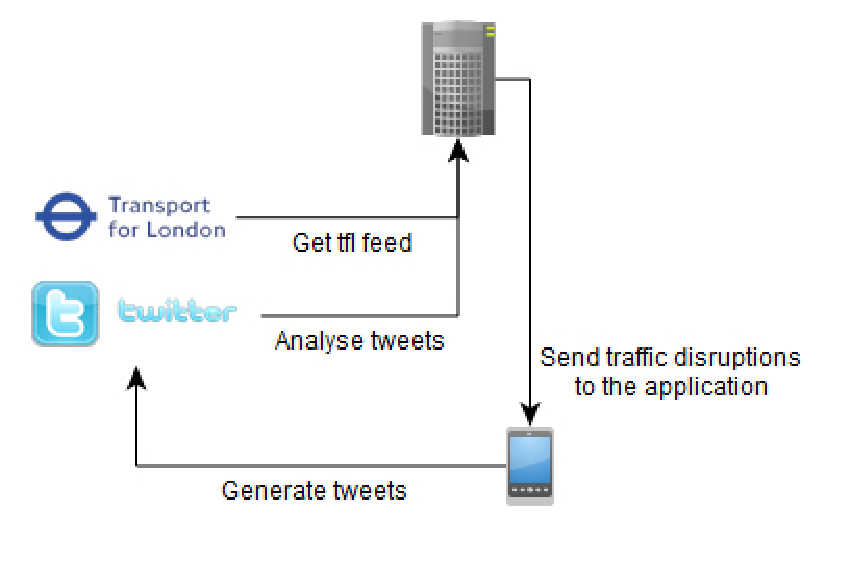
\includegraphics[width=0.7\textwidth]{images/draft_architecture.pdf}
\end{center}
\vspace{-20pt}
\caption{Data flow}
\end{figure}

The hosted application will retrieve traffic events from a Transport for London
(TfL)\cite{website:tfl_dev} data feed and a Twitter
feed\cite{website:twitter_dev} perodically. TfL provides a curated feed of
ongoing traffic disruptions in a structured format. Twitter provides us with a
torrent of unsorted tweets, from which relevant tweets must be extracted. 
Additionally, traffic disruptions reported from the mobile application can be
identified through the use of an identifier, enabling those messages to be
processed separately. To discover tweets that discuss traffic concepts,
document classification techniques will be utilised. As the message
classification algorithm improves, it is expected to be able to generate 
traffic disruptions that are reported only from Twitter, and not yet on TfL.

The mobile application must provide the commuter with a mechanism for discovering disruptions that may affect their route. This is to be provided through the use of a map based interface. The mobile application also must offer the user the ability to comment or describe an on going traffic disruption. The user interface for reporting disruptions must offer a quick and intuitive mechanism for describing a particular event, while also satisfying users that require more control over the messages published on their account.

The table below shows a breakdown of features ordered by their priority, feasibility and expected completion date. The smaller number in priority means more important to finish fast and in feasibility the smaller number means more achievable. Week 1 is considered to end on 27th of January, this leaves 8 weeks until the project deadline.

\begin{center}
\begin{tabular}{ | p{9cm} | c | c | p{1.8cm} | }
\hline
\multicolumn{4}{|c|}{\textbf{Mobile Application}} \\ \hline
\textbf{Feature} & \textbf{Priority} & \textbf{Feasibility} & \textbf{Due date} \\ \hline
\textbf{Report events}\newline
Report traffic disruption through the mobile application on Twitter. & 1 & 2 & Week 3 \\ \hline
\textbf{Present a list of classified and grouped tweets}\newline
Present to the user tweets identified as describing a traffic disruption,
clustered around an event. & 2 & 4 & Week 4 \\ \hline
\textbf{Show local disruption map}\newline
Show positions of known disruptions on a map. Enable the user to click on an event for further information. & 3 & 5 & Week 6 \\ \hline
\textbf{Stored Routes}\newline
Find and show disruptions for user defined stored routes. & 4 & 7 & Week 7 \\ \hline
\multicolumn{4}{|c|}{Minimum specifications for the mobile application are
features including and below priority 3.} \\ \hline
\end{tabular}
\end{center}
\begin{center}
\begin{tabular}{ | p{9cm} | c | c | p{1.8cm} | }
\hline
\multicolumn{4}{|c|}{\textbf{Server Hosted Application}} \\ \hline
\textbf{Feature} & \textbf{Priority} & \textbf{Feasibility} & \textbf{Due date} \\ \hline
\textbf{Store disruptions from TfL} \newline
Create a geographic database of live events from TfL. Evolve these database events with data from the feed, in order to have a current representation of the event. & 1 & 3 & Week 2 \\ \hline
\textbf{Store and categorise social data} \newline
For tweets with an explicit location, store them in a geographical database
table. And those tweets without this explicit information store them separately for later
analysis. & 2 & 2 & Week 2 \\ \hline
\textbf{Process mobile client reports} \newline
Take twitter messages reported from the mobile client and process these in a
separate pipeline. & 3 & 2 & Week 3 \\ \hline
\textbf{Classify tweets from Twitter with a simple classifier} \newline
Train a document classifier using a manually labeled training set to 
identify traffic related tweets. & 4 & 5 & Week 5 \\ \hline
\textbf{Identify traffic disruptions from Twitter} \newline
Inspect incoming traffic tweets and determine new non-TfL disruptions from
those. & 5 & 5 & Week 5 \\ \hline
\textbf{Geocoding of messages without explicit locations} \newline
Resolve geographic locations extracted from the message context. & 6 & 7 & Week 6 \\ \hline
\textbf{Enhance classification and clustering algorithms} \newline
From insight and data gained from initial classification and clustering
techniques, attempt to improve the accuracy of the results. & 7 & 9 & Week 7 \\ \hline
\multicolumn{4}{|c|}{Minimum specifications for the server application are
features including and below priority 4.} \\ \hline
\end{tabular}
\end{center}


\section{Development Methodology}
	\subsection{Development approach} 
To begin identifying an appropriate development methodology, it was necessary to firstly understand 
the project requirements. The project requirements and features were agreed over a number of 
meetings with the primary stakeholders.

The two most preferred development methodologies were 
Scrum and XP(Extreme Programming) which are both Agile methodologies. Scrum is an agile project management technique that focuses more 
on the management of software development projects. The product is completed in a series of one to 
four week iterations, or sprints as they are called. Before each sprint, a planning meeting is held 
to determine which features will be implemented during that sprint. Similarly, XP is an agile 
methodology which is designed for small, co-located teams aiming to get quality and productivity as 
high as possible. It does this through the use of rich, short, informal communication paths with 
emphasis on skill, discipline and understanding at the personal level, minimizing all intermediate 
work products. 

It was decided amongst the group that combining characteristics form both methods 
would be the most beneficial way, merely because they are complementary. Scrum focuses on the project management 
whereas XP on the programming part.\cite{ScrumXP}

Managing efficiently the development lifecycle of the project was a very 
important task for the team to work properly. Meetings with the supervisor took place each week 
where the project progress was thoroughly discussed as well as more feasible features to be 
implemented. In addition, various issues were constantly being brought up in order to provide solutions. Except from 
the meetings with the supervisor, the team had its own weekly meeting for keeping up with what 
everyone has been doing for the last week. New tasks were also assigned to members of the team. For 
every meeting an agenda was stored in an online document containing information about the team 
members absent, location, action items and topics to be discussed. In the end of the meeting tasks 
were assigned, managed or archived using an online visual board, similar to the Scrum Board, to 
encourage a more agile development.

As regards to the XP approach, it was proved that adopting 
some of its techniques would significantly improve the development process. More specifically, pair 
programming was effectively put in use. Team members where working in pairs whenever possible to 
develop a single feature. Additionally, XP promotes test-driven development. As mentioned in the 
first report, testing would be rather difficult due to the nature of the project being partly 
research based. However, essential tests were implemented in the server to validate the classifier 
as well as blackbox tests for the correctness and responsiveness of the rest API server. 

Throughout the development, various technologies had to be used and implemented. According to each 
members skills these elements were divided in such ways to effectively use the members previous 
experience. The team was also distributed to different design aspects of the project; however, more on the 
team structure will be discussed further on.

Lastly, for achieving parallel development between the mobile client application and the server, 
a mock server API was created, as mentioned in earlier reports that was accepting http requests and 
was returning static data sets to the client. 

\subsection{Testing} 
\subsubsection{Classifier Evaluation} 
Machine learning algorithms induce classifiers that depend on the training set, and there is a need for evaluation and statistical testing to assess the expected error rate of a classification algorithm, and even compare the expected error rates of two classification algorithms to be able to say which one is better. Evaluation can also be used as a guide for future improvements on the model. In order to evaluate the classifier several techniques have been used. The first technique is to generate a test set of tweets which their labels are already known. This test set has to be distinct from the train set which has been used to train the classifier. Afterward this test set is being classified by the classifier and the labels that it decides are being compared with their correct labels. The second technique is to calculate the accuracy of the classifier which measures the percentage of inputs in the test set that the classifier correctly labelled. To accomplish this, the build-in function of the package NLTK \emph{nltk.classify.accuracy()} has been used.

Additionally some more techniques have been implemented in order to get more
accurate evaluations and avoid possible `overfitting'. Note that there is a chance the classifier will become more accurate in the train set and less accurate in the test set with some parameter changes. This is when we have reached an "overfitting" to the train set. The first of these methods is the K-Fold Cross Validation. The dataset is split each time into K equally sized subsets, training and testing datasets, and then in n-th iteration (n=1..k) the n-th subset(testing set) is used for testing the classifier that has been built on all other remaining subsets. To present the result of this method the Confusion Matrix, which is a visualization tool typically used to present the results attained by a learner, has been created. Each column of the matrix represents the instances in a predicted class, while each row represents the instances in an actual class. Thus, the diagonal entries indicate labels that were correctly predicted, and the off-diagonal entries indicate errors. One benefit of a confusion matrix is that it is easy to see if the system is confusing two classes.

Finally, the Precision and Recall Rates can be calculated in order to ensure the results from the previous method. The recall and the precision can be derived from the confusion matrix by applying the following formulas:

\[ Precision\textsubscript{A} = tp\textsubscript{A}/(tp\textsubscript{A}+e\textsubscript{BA}+e\textsubscript{CA}) \]

\[ Recall\textsubscript{A} = tp\textsubscript{A}/(tp\textsubscript{A}+e\textsubscript{AB}+e\textsubscript{AC}) \]

Where the values "tp" and "e" are the elements of the confusion matrix as it can been seen on the figure~\ref{fig:confisionMatixCalc}.

\begin{figure}[h]
\begin{center}
\begin{tabular}{| l || c | c | c | }
    \hline
        & A & B & C  \\ \hline \hline
        A & tp\textsubscript{A} & e\textsubscript{AB} & e\textsubscript{AC} \\ \hline
        B & e\textsubscript{BA }& tp\textsubscript{B} & e\textsubscript{BC} \\\hline
        C & e\textsubscript{CA} & e\textsubscript{CB} & tp\textsubscript{C} \\\hline
    \end{tabular}
	\caption{A simple confusion matrix}
    \label{fig:confisionMatixCalc}
\end{center}
\end{figure}

While recall and precision rates can be individually used to determine the quality of a classifier, it is often more convenient to have a single measure to do the same assessment. The F\textsubscript{1} measure combines the recall and precision rates in a single equation:

\[ F\textsubscript{1} = 2*\frac{precision*recall}{precision+recall} \]

Because the labelled data was consisting of 1500 traffic tweets and 14505 non-traffic tweets, two different trainings and evaluations have been integrated. 

Firstly, the classifier was trained with 1000 traffic and 1000 non-traffic tweets. Then it was tested with 500 traffic and 500 non-traffic tweets. The metrics for this training are the following. 

Accuracy of the classifier:   0.87\\

Traffic precision:\hspace{15.5 mm}              0.842592592593\\
Traffic recall:\hspace{21.2 mm}                             0.91\\
Traffic F-measure:\hspace{12.8 mm}             0.875\\

Non-Traffic precision:\hspace{7.2 mm}        0.902173913043\\
Non-Traffic recall:\hspace{13 mm}            0.83\\
Non-Traffic F-measure:\hspace{4.6 mm}       0.864583333333\\

\begin{figure}[h]
\begin{center}
    \begin{tabular}{| l || c | c | }
    \hline
          & Non-Traffic & Traffic \\ \hline \hline
         Non-Traffic & 41.5\% & 8.5\% \\ \hline
         Traffic & 4.5\% & 45.5\% \\ \hline
    \end{tabular}
    \caption{Confusion Matrix with 1000 traffic and 1000 non-traffic tweets.}
    \label{fig:confusionMatrix1}
\end{center}
\end{figure}	

Secondly, the classifier was trained with 1000 traffic and 9670 non-traffic tweets. Afterward it was tested with 500 traffic and 4835 non-traffic tweets. The metrics for this training are the following. 

Accuracy of the classifier:   0.862605435801

Traffic precision:\hspace{15.5 mm}            0.401019541206\\
Traffic recall:\hspace{21.2 mm}               0.944\\
Traffic F-measure:\hspace{12.8 mm}         0.562909958259\\

Non-Traffic precision:\hspace{7.2 mm}         0.993265993266\\
Non-Traffic recall:\hspace{13 mm}           0.854188210962\\
Non-Traffic F-measure:\hspace{4.6 mm}         0.918492160569\\

\begin{figure}[h]
\begin{center}
    \begin{tabular}{| l || c | c | }
    \hline
          & Non-Traffic & Traffic \\ \hline \hline
        Non-Traffic & 77.4\% & 13.2\% \\ \hline
        Traffic & 0.5\% & 8.8\% \\ \hline
    \end{tabular}
    \caption{Confusion Matrix with 1000 traffic and 9670 non-traffic tweets.}
    \label{fig:confusionMatrix1}
\end{center}
\end{figure}
	
It can been observed from the confusion matrices, with the first training the classifier has been achieved a rather bad accuracy since 19\% of the non-traffic tweets are being classified wrong and 9\% of the traffic tweets are being classified wrong. On the other hand, with the second training the traffic tweets error has been almost halved to 5\% resulting a more accurate classification for the traffic tweets even if the global accuracy dropped by 1\%. That means the classifier may classified some traffic tweets as non-traffic but it classified much less non-traffic tweets as traffic. Note that all the above results have been taken after the implementation of the normalization. During the first evaluation, before the pre-processing, the accuracy of the classifier was 77\%. However after the application of the normalization�s techniques the accuracy has been increased by 10\%!

As it has been mentioned before, a strong motivation for the creation of this project was the previous work of Dr. Luke Dicken in the same field. Having that in mind, it has been considered necessary to compare the accuracy of the classifier and the efficient of the server with his work. So in addition to the previous evaluation results, several metrics have been calculated in order to find the efficient of the classifier and the server. Those metrics are being presented in the figures below.

\begin{figure}[h]
\begin{center}
    \begin{tabular}{| c | c | c | }
    \hline
        Total Number of Tweets  & Non-Traffic & Traffic \\ \hline 
        71036 & 68096(95.86\%) & 2940(4.14\%) \\ \hline
    \end{tabular}
    \caption{Comparison of Traffic and Non-Traffic Tweets.}
    \label{fig:metrics1}
\end{center}
\end{figure}
	
\begin{figure}[h]
\begin{center}
    \begin{tabular}{| c | c | c | }
    \hline
        Geo-Tagged  & Geo-Tagged Genuine & Geo-Tagged from the 
Geolocation Resolver \\ \hline 
        314(10.68\%) & 136(4.63\%) & 178(6.05\%) \\ \hline
    \end{tabular}
    \caption{Tweets with geolocation from the 2940 traffic tweets.}
    \label{fig:metrics2}
\end{center}
\end{figure}


\begin{figure}[h]
Overall inferred rates:
\begin{center}
    \begin{tabular}{| l || c | c | c |}
    \hline
        & Filtered & Traffic & Geo-Tagged and Traffic\\ \hline \hline
        each minute & 13.3 & 0.5 & 0.06 \\ \hline
		each 5 mins & 66.7 &  2.7 & 0.3 \\ \hline
		each hour & 800 & 32.7 & 3.5 \\ \hline
    \end{tabular}
    \caption{Averages are over total 5400 minutes (90 hours) of up-time.}
    \label{fig:metrics3}
\end{center}
\end{figure}


\subsubsection{Functional/Integration Testing}
One of the most important parts of the project was the server API interface. A lot of requests will 
be coming from the mobile application and it must be confirmed that the server interface can handle 
them but also return the expected results using the expected format. In order to test the server 
interface the Apache JMeter desktop application was used. This software is designed to load test 
functional behaviour and measure the performance of static and dynamic recourses. Using JMeter 
proved to be a very effective way to test the servers interface. Various test plans where created 
testing every GET or POST request available to use through the API. These plans where created for 
both the server and the mock server that are running on ports 55004 and 55003 accordingly. More 
tests were implemented to ensure that the server was returning the correct messages and response 
codes when it was encountering an error. In addition, invalid requests to the server had also been 
checked for error handling and if the error messages were displayed correctly into the screen. For 
each request, the content-type was also checked if it evaluates as JSON. This process was really 
helpful because it was very easy later on to check whether new features implemented or code 
refactoring were actually breaking the API. All the test plan configuration settings have been saved 
in the project repository as a .jmx file. 

\subsubsection{Unit Testing} 



\section{Revision Control}
	Management of source-code, documentation and binary files can be tedious for an individual, but when you consider a team working on a set of files, tracking changes and version becomes close to impossible.

While many different approaches are used to track files, most revision control systems offer
similar basic functionality. This main functionality could be described under
the title ‘collaboration’, enabling multiple individuals to work on as set of
files while ensuring changes don’t get lost and enabling tracking of versions.
Modern systems offer powerful features such as verifiable histories, ability to integrate with deployment, test and code review systems and the ability to add rules to enforce corporate policy and process.

Of the options available, the chosen system had to satisfy a number of requirements. The system had to be free and preferably open-source, work well in a disconnected environment, have good documentation and also beneficial if this tool is in common use. Git\cite{website:git_scm}, the open-source distributed revision control system used by many major projects including the Linux Kernel, Google’s Android, Eclipse and Ruby on Rails seemed to meet the teams requirements. Additionally a number of team members have previous experience using the tool, which will lessen the initial learning curve.

The distributed nature of Git means a centralised ‘server’ is not necessary, but for convenience Github\cite{website:github} an online hosting service for git is being utilised. In addition to simply hosting the repository, Github offers a simple user interface for browsing the history, project bug-tracking and wiki for documentation, and is free for public projects with less the 300mb of history. There is however a downside to using Github, we lose the ability to write scripts to interface with the git hooks framework (on the server). 

From the beginning of the project it was agreed that all data will exist outside of the repository. This was enforced initially by creating a defined directory structure for the repository and secondly by creating a ‘.gitignore’ file in the root of the repository to list file types to be not tracked by default.  

To extract as much value as possible from revision control it is important to
make commit messages as concise and descriptive as possible. The book Pro
Git\cite{website:pro_git_ch2} describes a good commit as the following; break
the message into a brief 50 character summary, a new line and a more detailed
description. Enforcing good commit messages will help any team member to
quickly look at the commit log and understand the current state of development.
It is also important not get too wrapped up in these aspects, and keep the development somewhat agile.

The team’s repository is available at: \url{https://github.com/johnflan/Twitter-4-Traffic}
\pagebreak 


\section{References}
	\def\refname{}
	\bibliography{references}
	\bibliographystyle{plain}

\end{document}
